\label{sec:det}
The Dynamic Event Tree approach (DET) is a well-known methodology, developed based on the Static (or Classical) Event Tree (ET) technique. In the ET approach, starting from an initiating event (i.e. accident event), all possible final outcomes of the accident scenario are obtained by assembling of status combinations of the system (e.g., responsiveness of components/sub-systems) that might impact the final outcome. This leads to the classical tree structure. Each branch end (accident scenario outcome) could be characterized therefore by the status of the components/subsystem that leads to such outcome. The probability of such outcome is the product of the probability of the components/subsystems to be in the corresponding status. The two main disadvantages of this approach are that timing/sequencing of events and system dynamic responses are not explicitly accounted for in the analysis.

In order to overcome these limitations a “dynamic” approach is necessary. The DET technique is, in fact, capable of simulating the probabilistic system evolution in a consistent way with respect to temporal evolution of the accident scenarios~\cite{alfonsiPSA}~\cite{ADAPTHakobyan}. This means the DET enables a feedback mechanism between the accident scenarios defined by probability of events over the accident timeline, and the dynamic response of the system. In the DET approach, a single initiating event (root) leads to multiple final outcomes. The branching occurs at user specified times/conditions and/or when an action is required by the operator and/or by the control system. The branching process creates a deterministic sequence of events based on the time of their occurrence (see fig.~\ref{fig:DET_schemeFlow}). The criteria for branching are generally geared toward providing complete coverage of all-possible scenarios. The number of branches (dynamic sequences) can become very large very quickly. For this reason independent branches are simulated in parallel.

This approach leads to a more realistic analysis of the considered system (e.g., NPP) than the classical static Event Tree. General Dynamic Probabilistic Risk Assessment methodologies, among which DET, are designed to consider the timing of single events explicitly, which can become extremely important especially when non linearity of the system response might alter the scenario evolution.

The main idea of this methodology is to let a system code (i.e., RELAP-7) to determine the pathway of an accident scenario within a probabilistic “environment” rather than statically combining the effects of all possible component status toward the final outcome of the accident scenario.
\begin{figure}[h]
  \centering
     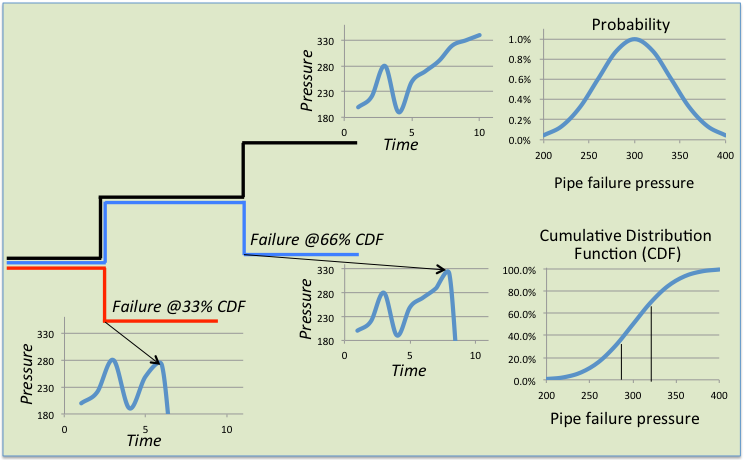
\includegraphics[width=0.73\textwidth]{figures/DET_schemeFlow.png}
  \caption{Dynamic Event Tree Conceptual Scheme.}
   \label{fig:DET_schemeFlow}
\end{figure}

From a simulation point of view, a DET analysis starts with a single simulation that, most likely, represents an abnormal condition of the NPP immediately after an initiating event (e.g., fire, flooding, etc.). Every time during the simulation, the system evolution leads to a probabilistic event (e.g., failure of a relief valve, recovery of a safety feature, etc.), several simulation branches are spawned. Each simulation carries along one of the possible outcomes of the probabilistic event and the associated event probability. As illustrated in fig.~\ref{fig:DET_schemeFlow}, after an initiating event, which leads to an abnormal condition of the system, the simulation follows the accident sequence and a pipe status is affected by a probability of failure (i.e., pipe failure probability as a function of the internal pressure) described by a Probabilistic Distribution Function (PDF) and a corresponding Cumulative Distribution Function (CDF). The user provides a grid of probability thresholds, with respect the CDFs of the uncertain parameters (in this case on the failure pressure). Every time the simulation detects a pressure corresponding to a threshold in the probability grid, a new set of simulation branches are generated (i.e., a branch where the pipe is damaged and another where nothing happened).

In general, each sequence continues until another event occurs and a new set of branches is spawned. The simulation ends when an exit condition or a maximum mission time is reached. At the end of the DET analysis, all the branches (that represent all the possible system evolutions) are assembled in order to create a set of completed histories.
